%% ------------- Portuguese version ------------
\documentclass{sbrt}
\usepackage[english,brazil]{babel}
\usepackage[utf8]{inputenc}
\newtheorem{theorem}{Teorema}
\usepackage{amsmath}
\usepackage{graphicx}
\usepackage[colorlinks=true, allcolors=blue]{hyperref}
\usepackage{float} % for [H] option
\usepackage{amsmath} % for mathematical equations
\usepackage{multirow}
\usepackage{booktabs}

%% ---------------------------------------------

%% If writing in English, remove the lines above
%% and uncomment the lines below

%% ------------- English version ---------------
%\documentclass[english]{sbrt}
%\usepackage[english]{babel}
%\usepackage[utf8]{inputenc}
%\newtheorem{theorem}{Theorem}
%% ---------------------------------------------

\begin{document}

\title{Classification Project}
\author{João Victor, Ryan Reis, Valdinei Rodrigues}

\maketitle




\title{Classification problem}
\author{João Victor, Ryan Reis, Valdinei Rodrigues}


\section{Introduction}
This work addresses two distinct parts. In Part I, we use the MNIST dataset, including versions with Gaussian noise, to evaluate the robustness of three scikit-learn classifiers (Naive Bayes, Decision Tree, and SVM). The results are presented in terms of accuracy under different training and testing conditions. Furthermore, a study of the complexity of the sample is carried out to determine the necessary number of training examples to achieve a given accuracy. In Part II, we select our own dataset for classification, excluding the insertion of noise, and repeat the evaluation of the chosen classifiers, focusing only on the matched condition. Again, an analysis of the sample complexity is performed for the best classifier.



\section{Part 1}

In this project phase, we will work with the MNIST dataset, comprising zip code digits, enhanced with Gaussian noise to achieve a peak signal-to-noise ratio (PSNR) of 10 dB across the training, testing, and validation sets. With the test set containing 20\% of the total dataset examples and being disjoint from the others. divided into two parts, on part involves assessing the robustness of selected classifiers to mismatched training and testing sets, comparing models trained with and without noise. and the other requires constructing a sample complexity curve for the best-performing machine learning algorithm using only the original MNIST data, revealing the number of training examples needed for satisfactory accuracy. Both deliverables aim to elucidate the efficacy and performance characteristics of the chosen classifiers under various conditions.

\subsection{PSNR generator}

This is the mathematical function that generates the PSNR:

\begin{figure}[H]
    \centering
    \[
    \text{PSNR} = 10 \cdot \log_{10}\left(\frac{\text{MAX}^2}{\text{MSE}}\right)
    \]
    
    \[
    \frac{\text{PSNR}}{10} = \log_{10}\left(\frac{\text{MAX}^2}{\text{MSE}}\right)
    \]
    
    \[
    10^{\frac{\text{PSNR}}{10}} = \frac{\text{MAX}^2}{\text{MSE}}
    \]
    
    \[
    \text{MSE} = \frac{\text{MAX}^2}{10^{\frac{\text{PSNR}}{10}}}
    \]
    
    The value of MAX is 255 and we want a PSNR of 10dB, so the equation is:
    
    \[
    \text{MSE} = \frac{255^2}{10^{\frac{10}{10}}} = 6502.5
    \]
    \caption{PSNR Calculation}
    \label{fig:psnr-calculation}
\end{figure}

\subsection{pre-processing}

We begin by importing necessary libraries and loading the MNIST dataset using Scikit-learn. The dataset is split into training, validation, and test sets separated at 70\%, 10\% and 20\% respectively. Additionally, we introduce a noisy version of the dataset by adding Gaussian noise with a predefined peak signal-to-noise ratio (PSNR) to simulate noisy real-world conditions.

\subsection{Training dataset with and without noise}

\subsubsection{Naive Bayes Classification}

We employ Gaussian Naive Bayes classifier and perform grid search for hyperparameter tuning on the validation set. The best parameters obtained are used to train the model on the original MNIST dataset. The trained model is evaluated on the test set, and results are visualized using a confusion matrix and classification report, and we got the following accuracy.

\begin{table}[htbp]
  \centering
  \caption{Naive Bayes Model Performance}
    \begin{tabular}{lcc}
    \toprule
    \textbf{Training Condition} & \textbf{Testing Condition} & \textbf{Accuracy} \\
    \midrule
    No Noise & No Noise & 0.82 \\
    No Noise & With Noise & 0.61 \\
    With Noise & No Noise & 0.79 \\
    With Noise & With Noise & 0.84 \\
    \bottomrule
    \end{tabular}%
  \label{tab:addlabel}%
\end{table}%

\subsubsection{Decision Tree Classification}

We utilize a Decision Tree classifier and perform grid search for hyperparameter optimization on the validation set. The best parameters are used to train the model on the original MNIST dataset, followed by evaluation on the test set. Additionally, we visualize the trained decision tree, and we got the following accuracy.

\begin{table}[htbp]
  \centering
  \caption{Decision Tree Model Performance}
    \begin{tabular}{lcc}
    \toprule
    \textbf{Training Condition} & \textbf{Testing Condition} & \textbf{Accuracy} \\
    \midrule
    No Noise & No Noise & 0.88 \\
    No Noise & With Noise & 0.33 \\
    With Noise & No Noise & 0.81 \\
    With Noise & With Noise & 0.66 \\
    \bottomrule
    \end{tabular}%
  \label{tab:addlabel}%
\end{table}%

\subsubsection{SVM}

We employ a Support Vector Machine (SVM) classifier with grid search for hyperparameter optimization on the validation set. The best parameters are used to train the model on the original MNIST dataset, and evaluation is performed on the test set, and we got the following accuracy:

\begin{table}[htbp]
  \centering
  \caption{SVM Model Performance}
    \begin{tabular}{lcc}
    \toprule
    \textbf{Training Condition} & \textbf{Testing Condition} & \textbf{Accuracy} \\
    \midrule
    No Noise & No Noise & 0.98 \\
    No Noise & With Noise & 0.68 \\
    With Noise & No Noise & 0.96 \\
    With Noise & With Noise & 0.95 \\
    \bottomrule
    \end{tabular}%
  \label{tab:addlabel}%
\end{table}%



All these values give us the following table:

So after comparing the performance of Naive-Bayes, Decision Tree, and Support Vector Machine (SVM) models both with and without noise, we have chosen the SVM model due to its consistently high accuracy across both scenarios. With an accuracy of 98.4\% without noise and 95.5\% with noise, SVM demonstrates robustness and effectiveness in classification tasks, making it the preferred choice for our application.

\section{Sample complexity}

Below, we generate a sample complexity curve for the
previously identified best-performing SVM model. This curve
illustrates how the size of the training set impacts the mo-
del’s performance. The resulting accuracy scores for different
sample sizes are as follows:

\begin{table}[htbp]
  \centering
  \caption{Accuracy with Different Training Samples}
    \begin{tabular}{rr}
    \toprule
    \textbf{Training Samples} & \textbf{Accuracy} \\
    \midrule
    100   & 0.7058571428571428 \\
    500   & 0.8858571428571429 \\
    1000  & 0.923 \\
    5000  & 0.9595714285714285 \\
    10000 & 0.9704285714285714 \\
    15000 & 0.9747142857142858 \\
    20000 & 0.9778571428571429 \\
    25000 & 0.9797142857142858 \\
    30000 & 0.9807142857142858 \\
    35000 & 0.9841428571428571 \\
    40000 & 0.9818571428571429 \\
    49000 & 0.9841428571428571 \\
    \bottomrule
    \end{tabular}%
  \label{tab:addlabel}%
\end{table}%

These results are visualized in the plot below, depicting the
number of training samples versus the test accuracy.

\begin{figure}[H]
    \centering
    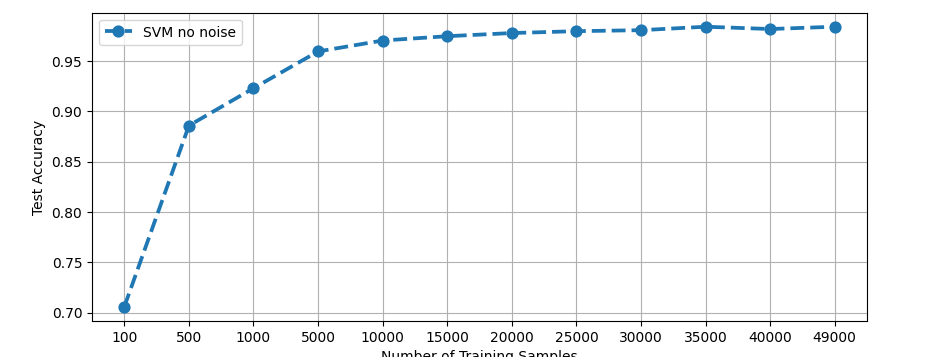
\includegraphics[width=0.6\textwidth]{images/complexity_curve_p1.png}
    \caption{Data standardization}
    \label{fig:example}
\end{figure}


\section{Part 2}

In this section, we delve into the part 2 of the project, data treatment, and pre-processing steps conducted on the chosen dataset "credit\_data.csv". This dataset, simulates credit agency data, with attributes including income, age, loan, and a class column indicating default status (1 for default, 0 for non-default).

\subsection{Initial Analisis}

We initiated our exploration by loading the dataset using the Pandas library and performing a preliminary analysis. Utilizing the describe() function, we obtained descriptive statistics, revealing potential inconsistencies such as negative age values. These inconsistencies were addressed to ensure the robustness of our subsequent modeling steps.

\begin{figure}[H]
    \centering
    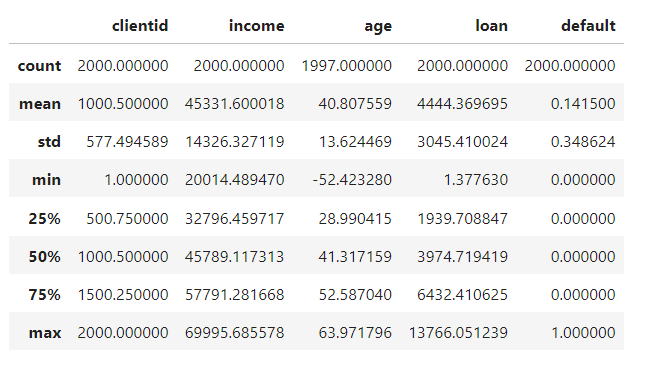
\includegraphics[width=0.4\textwidth]{images/table_1.png}
    \caption{Table with incorrect age value}
    \label{fig:example}
\end{figure}


After this result we deleted the incorrect data and filled the gap with the data average of the rest of the data, and after this adjust we got a more consistent result.

\subsection{Pre-Processing}

Prior to model training, we partitioned the dataset into predictors (X\_credit) and classes (y\_credit). Subsequently, we standardized the predictors using the StandardScaler to ensure uniformity and facilitate the performance of machine learning algorithms. This standardization process transforms the data to have a mean of zero and a standard deviation of one, enhancing algorithm performance, particularly for those assuming normally distributed, scaled data.

\begin{figure}[htbp]
    \centering
    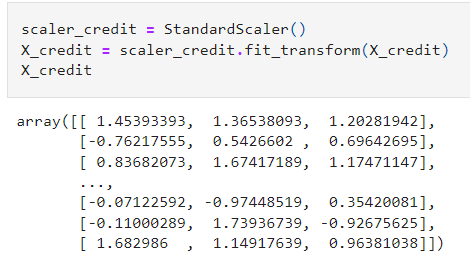
\includegraphics[width=0.4\textwidth]{images/Standadization.png}
    \caption{Data standardization}
    \label{fig:example}
\end{figure}


\subsection{Train-Test-Split}

Following pre-processing, we divided the data into training and testing sets, allocating 70\% for training and 30\% for testing. This partitioning step is crucial for accurate model evaluation and generalization to new data.

These initial steps laid the foundation for subsequent modeling, enabling us to apply various machine learning algorithms to predict credit default status effectively.

\subsubsection{Naive Bayes}

Before training the model, let's check the best hyperparameters for the Naive bayes algorithm. GridSearchCV is a popular technique in machine learning used to find the best hyperparameters for a model. It works by creating a "grid" of possible hyperparameters and testing all possible combinations of these hyperparameters, using cross-validation to evaluate the performance of each combination.

With these parameters we got the following result as the confusion matrix:

\begin{figure}[H]
    \centering
    \includegraphics[width=0.35\textwidth]{images/Matriz_de_confusão.png}
    \caption{Confusion matrix Naive Bayes}
    \label{fig:example}
\end{figure}\textbf{}

with an accuracy of 0.935\%

\subsubsection{Decision Tree}

For the decision Tree classificator we got the following confusion matrix:

\begin{figure}[H]
    \centering
    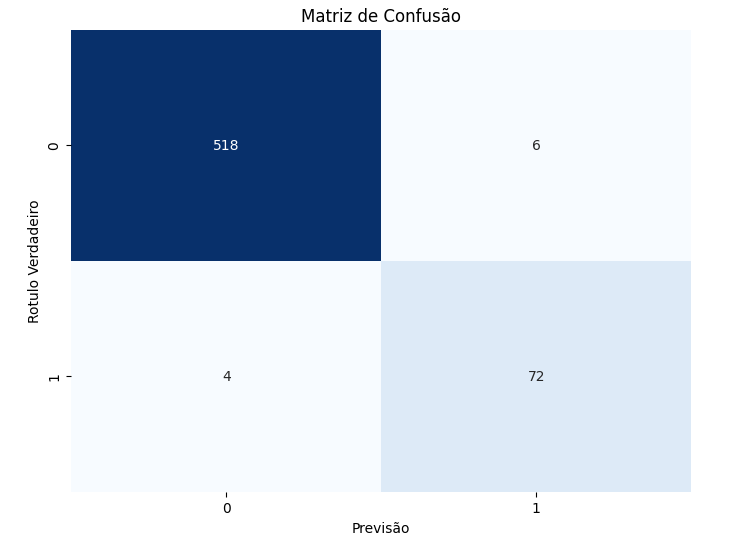
\includegraphics[width=0.35\textwidth]{images/confusion-matrix-decision-tree.png}
    \caption{Confusion matrix decision tree}
    \label{fig:example}
\end{figure}\textbf{}

With an accuracy of 0.983\%

\subsubsection{SVM}

For the SVM classificator we got the following confusion matrix

\begin{figure}[H]
    \centering
    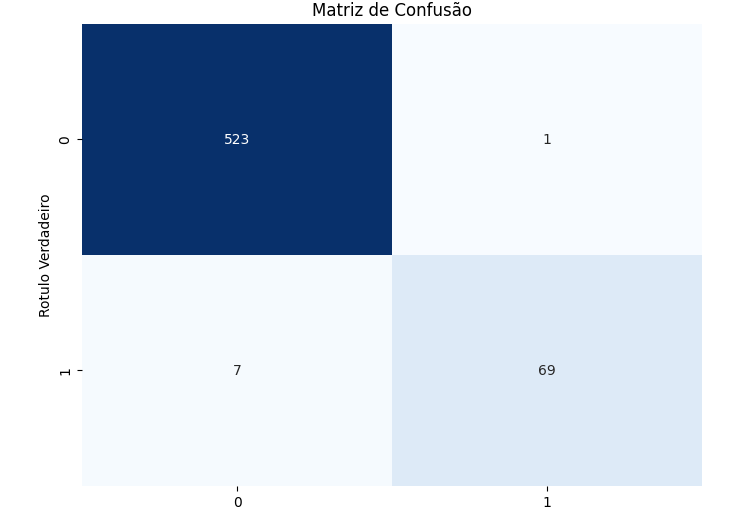
\includegraphics[width=0.3\textwidth]{images/confusion-matrix-svm.png}
    \caption{Confusion matrix SVM}
    \label{fig:example}
\end{figure}\textbf{}

With an accuracy of 0.986\%


\subsubsection{conclusion from the trai-test phase}

The results obtained show an accuracy above 90\% in the three models tested, with Decision Tree and SVM achieving almost equivalent results. However, when analyzing the detailed statistics, we observed that SVM slightly outperforms Decision Tree in terms of overall accuracy, precision for the positive class and F1-Score for the same class. On the other hand, the decision tree shows slightly better recall for the positive class. Therefore, the choice between these models will depend on the specific needs of the problem and the priority evaluation metrics.

\section{Sample complexity}

Below, we generate a sample complexity curve for the previously identified best-performing SVM model. This curve illustrates how the size of the training set impacts the model's performance.
The resulting accuracy scores for different sample sizes are as follows:

\begin{table}[H]
  \centering
  \caption{Accuracy with Different Training Samples}
    \begin{tabular}{rr}
    \toprule
    \textbf{Training Samples} & \textbf{Accuracy} \\
    \midrule
    100   & 0.9433 \\
    200   & 0.9667 \\
    300   & 0.9717 \\
    400   & 0.9750 \\
    500   & 0.9800 \\
    600   & 0.9867 \\
    700   & 0.9867 \\
    800   & 0.9817 \\
    900   & 0.9850 \\
    1000  & 0.9883 \\
    1100  & 0.9883 \\
    1200  & 0.9883 \\
    1300  & 0.9867 \\
    1400  & 0.9867 \\
    \bottomrule
    \end{tabular}%
  \label{tab:addlabel}%
\end{table}%

These results are visualized in the plot below, depicting the number of training samples versus the test accuracy.

\begin{figure}[H]
    \centering
    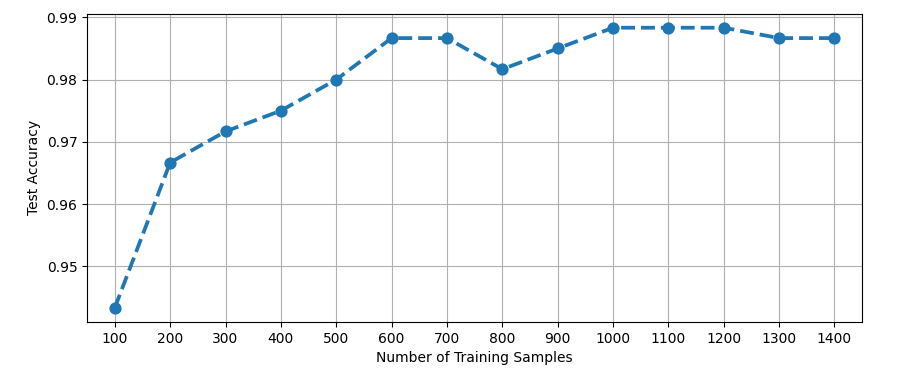
\includegraphics[width=0.5\textwidth]{images/complexity_curve.png}
    \caption{Complexity curve}
    \label{fig:example}
\end{figure}\textbf{}


\end{document}
